\documentclass[12pt]{report}

\usepackage{amsmath} % loads AMS-Math package
\usepackage{euscript}
\usepackage{amssymb}
\usepackage{epsfig} % allows PostScript files
\usepackage{graphicx}
\usepackage{multirow}
\usepackage{listings} % allows lstlisting environment
\usepackage{moreverb} % allows listinginput environment
\usepackage{vmargin} % allows better margins
\usepackage{color}
\usepackage{mcode}
\setpapersize{USletter} % sets the paper size
\allowdisplaybreaks[1]
\setmarginsrb{1in}{0.7in}{1in}{1in}{12pt}{11mm}{0pt}{11mm} %sets margins


\title{\LaTeX \ Title }

\author{Alex Beutel  \\
{\small\em \copyright \  Draft date \today }}

 \date{ }

 %\abstract{Some bullshit}

\begin{document}

\maketitle
\begin{abstract}
	blah blah blah
\end{abstract}
 %\addcontentsline{toc}{chapter}{Contents}
\pagenumbering{roman}
\tableofcontents
\listoffigures
\listoftables

\pagestyle{headings}
\pagenumbering{arabic}

\pagestyle{plain}

\chapter{Introduction}

\input{writing/intro}

\chapter{Chaos Theory}

\section{Nonlinear Dynamics}
\label{sec: Nonlinear Dynamics}
\input{writing/nonlinearDynamics}

\section{Chaos ``Proof"}
\label{sec: Chaos ``Proof"}
\input{writing/chaosProof}

\section{Nonlinear Methods}
\label{sec: Nonlinear Methods}
\input{writing/nonlinearMethods}

\chapter{Experimental Setup}

\section{RL Diode Circuit}
\label{sec:RL Diode Circuit}
\input{writing/RLDiodeCircuit}

\section{Picoscope}
\label{sec:Picoscope}
\input{writing/picoscope}

\section{Oscilloscope}
\label{sec:Oscilloscope}
\input{writing/oscilloscope}

\chapter{Experimental Procedure}
\input{writing/experimentalProcedure}

\chapter{Results}

\section{Data Analysis} % (fold)
\label{sec:Data Analysis}

	\begin{figure}[h]
		\centering
		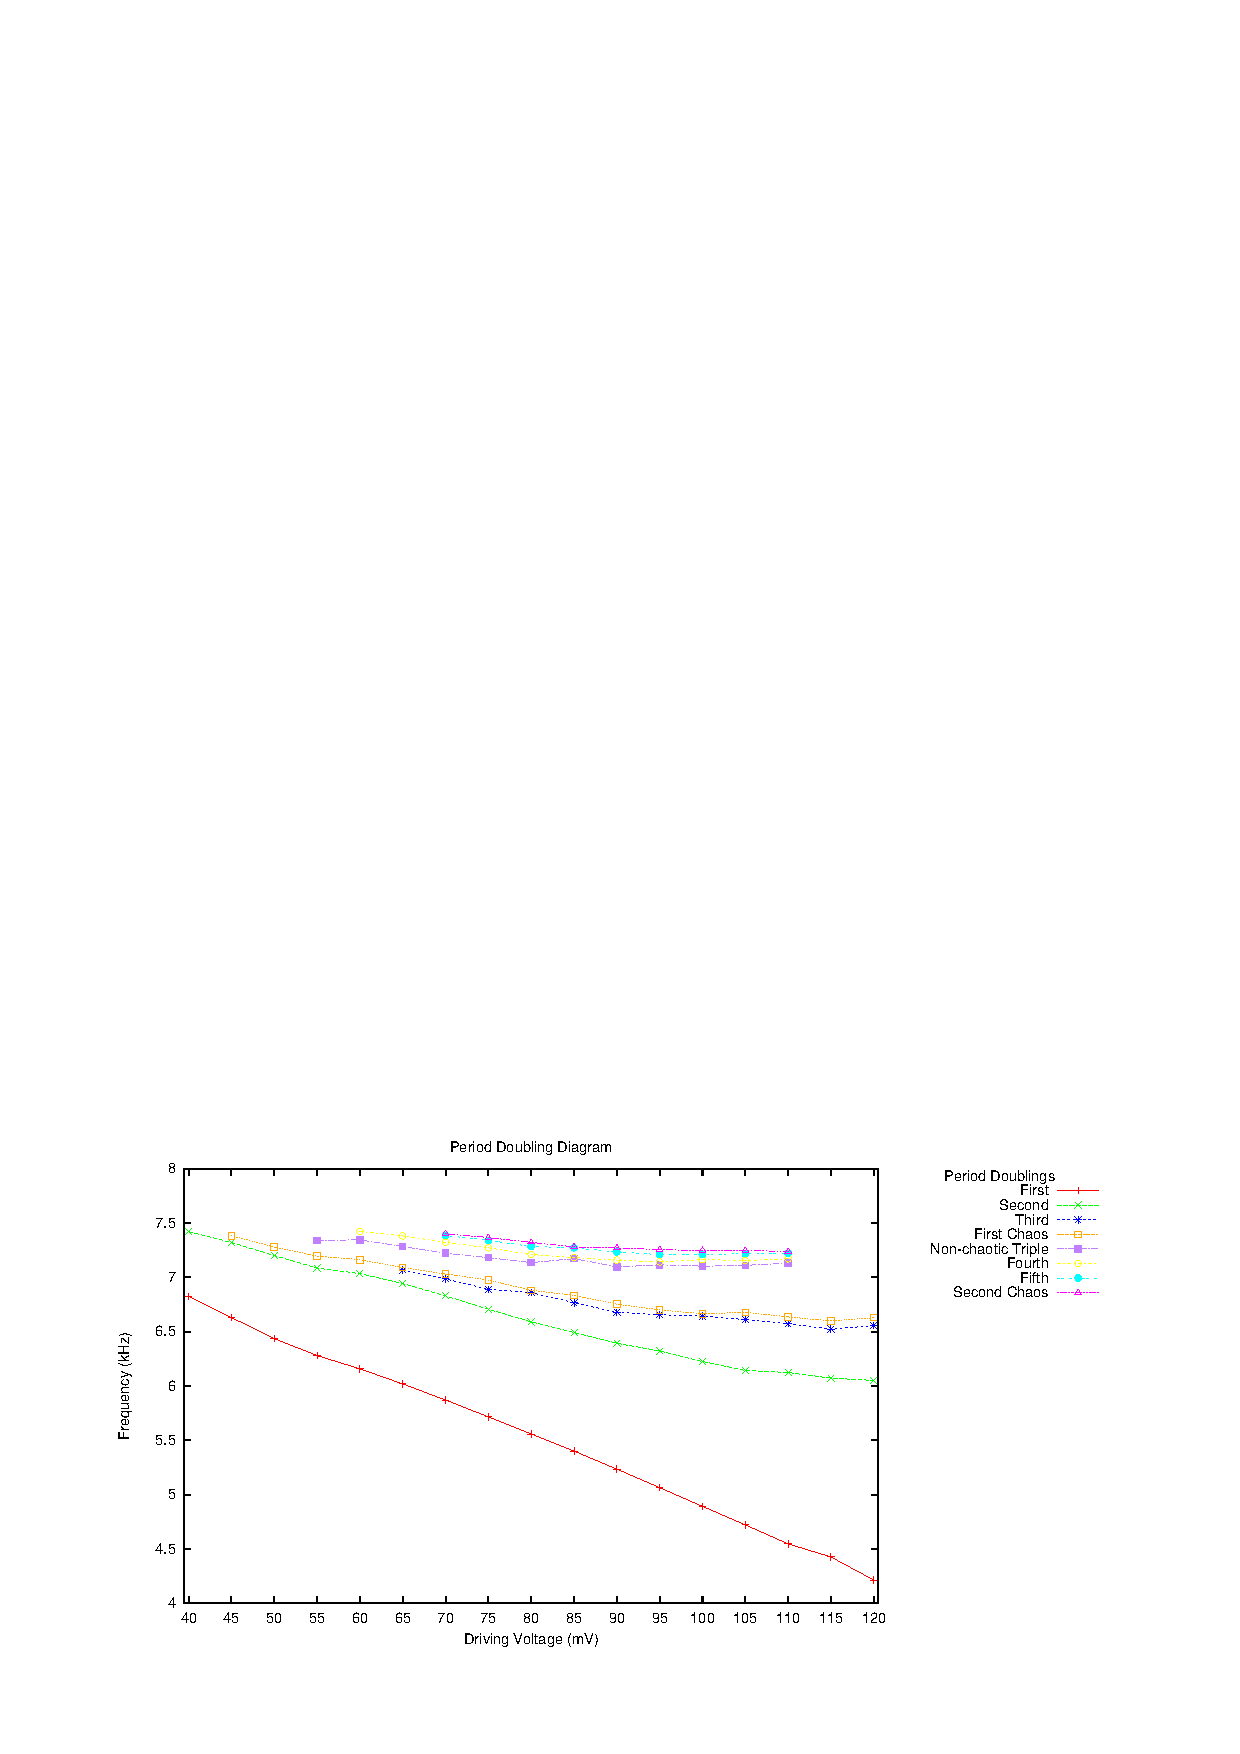
\includegraphics{plots/general.pdf}
		\label{fig:periodDoubling}
		\caption{Period Doubling}
	\end{figure}

\input{writing/periodDoubling}

	\begin{figure}[h]
		\centering
		% GNUPLOT: LaTeX picture
\setlength{\unitlength}{0.240900pt}
\ifx\plotpoint\undefined\newsavebox{\plotpoint}\fi
\sbox{\plotpoint}{\rule[-0.200pt]{0.400pt}{0.400pt}}%
\begin{picture}(1500,900)(0,0)
\sbox{\plotpoint}{\rule[-0.200pt]{0.400pt}{0.400pt}}%
\put(191.0,131.0){\rule[-0.200pt]{4.818pt}{0.400pt}}
\put(171,131){\makebox(0,0)[r]{ 60}}
\put(1429.0,131.0){\rule[-0.200pt]{4.818pt}{0.400pt}}
\put(191.0,203.0){\rule[-0.200pt]{4.818pt}{0.400pt}}
\put(171,203){\makebox(0,0)[r]{ 70}}
\put(1429.0,203.0){\rule[-0.200pt]{4.818pt}{0.400pt}}
\put(191.0,274.0){\rule[-0.200pt]{4.818pt}{0.400pt}}
\put(171,274){\makebox(0,0)[r]{ 80}}
\put(1429.0,274.0){\rule[-0.200pt]{4.818pt}{0.400pt}}
\put(191.0,346.0){\rule[-0.200pt]{4.818pt}{0.400pt}}
\put(171,346){\makebox(0,0)[r]{ 90}}
\put(1429.0,346.0){\rule[-0.200pt]{4.818pt}{0.400pt}}
\put(191.0,418.0){\rule[-0.200pt]{4.818pt}{0.400pt}}
\put(171,418){\makebox(0,0)[r]{ 100}}
\put(1429.0,418.0){\rule[-0.200pt]{4.818pt}{0.400pt}}
\put(191.0,489.0){\rule[-0.200pt]{4.818pt}{0.400pt}}
\put(171,489){\makebox(0,0)[r]{ 110}}
\put(1429.0,489.0){\rule[-0.200pt]{4.818pt}{0.400pt}}
\put(191.0,561.0){\rule[-0.200pt]{4.818pt}{0.400pt}}
\put(171,561){\makebox(0,0)[r]{ 120}}
\put(1429.0,561.0){\rule[-0.200pt]{4.818pt}{0.400pt}}
\put(191.0,633.0){\rule[-0.200pt]{4.818pt}{0.400pt}}
\put(171,633){\makebox(0,0)[r]{ 130}}
\put(1429.0,633.0){\rule[-0.200pt]{4.818pt}{0.400pt}}
\put(191.0,704.0){\rule[-0.200pt]{4.818pt}{0.400pt}}
\put(171,704){\makebox(0,0)[r]{ 140}}
\put(1429.0,704.0){\rule[-0.200pt]{4.818pt}{0.400pt}}
\put(191.0,776.0){\rule[-0.200pt]{4.818pt}{0.400pt}}
\put(171,776){\makebox(0,0)[r]{ 150}}
\put(1429.0,776.0){\rule[-0.200pt]{4.818pt}{0.400pt}}
\put(191.0,131.0){\rule[-0.200pt]{0.400pt}{4.818pt}}
\put(191,90){\makebox(0,0){ 12}}
\put(191.0,756.0){\rule[-0.200pt]{0.400pt}{4.818pt}}
\put(401.0,131.0){\rule[-0.200pt]{0.400pt}{4.818pt}}
\put(401,90){\makebox(0,0){ 14}}
\put(401.0,756.0){\rule[-0.200pt]{0.400pt}{4.818pt}}
\put(610.0,131.0){\rule[-0.200pt]{0.400pt}{4.818pt}}
\put(610,90){\makebox(0,0){ 16}}
\put(610.0,756.0){\rule[-0.200pt]{0.400pt}{4.818pt}}
\put(820.0,131.0){\rule[-0.200pt]{0.400pt}{4.818pt}}
\put(820,90){\makebox(0,0){ 18}}
\put(820.0,756.0){\rule[-0.200pt]{0.400pt}{4.818pt}}
\put(1030.0,131.0){\rule[-0.200pt]{0.400pt}{4.818pt}}
\put(1030,90){\makebox(0,0){ 20}}
\put(1030.0,756.0){\rule[-0.200pt]{0.400pt}{4.818pt}}
\put(1239.0,131.0){\rule[-0.200pt]{0.400pt}{4.818pt}}
\put(1239,90){\makebox(0,0){ 22}}
\put(1239.0,756.0){\rule[-0.200pt]{0.400pt}{4.818pt}}
\put(1449.0,131.0){\rule[-0.200pt]{0.400pt}{4.818pt}}
\put(1449,90){\makebox(0,0){ 24}}
\put(1449.0,756.0){\rule[-0.200pt]{0.400pt}{4.818pt}}
\put(191.0,131.0){\rule[-0.200pt]{0.400pt}{155.380pt}}
\put(191.0,131.0){\rule[-0.200pt]{303.052pt}{0.400pt}}
\put(1449.0,131.0){\rule[-0.200pt]{0.400pt}{155.380pt}}
\put(191.0,776.0){\rule[-0.200pt]{303.052pt}{0.400pt}}
\put(50,453){\makebox(0,0){\shortstack{V$_{\rm resistor}$\\(mV)}}}
\put(820,29){\makebox(0,0){V$_{\rm drive}$ (mV)}}
\put(820,838){\makebox(0,0){Bifurcation for 80khz}}
\put(243,156){\rule{1pt}{1pt}}
\put(327,188){\rule{1pt}{1pt}}
\put(359,203){\rule{1pt}{1pt}}
\put(422,217){\rule{1pt}{1pt}}
\put(464,231){\rule{1pt}{1pt}}
\put(537,253){\rule{1pt}{1pt}}
\put(621,278){\rule{1pt}{1pt}}
\put(726,303){\rule{1pt}{1pt}}
\put(747,307){\rule{1pt}{1pt}}
\put(768,328){\rule{1pt}{1pt}}
\put(768,292){\rule{1pt}{1pt}}
\put(799,342){\rule{1pt}{1pt}}
\put(799,282){\rule{1pt}{1pt}}
\put(830,364){\rule{1pt}{1pt}}
\put(830,253){\rule{1pt}{1pt}}
\put(872,375){\rule{1pt}{1pt}}
\put(872,239){\rule{1pt}{1pt}}
\put(914,393){\rule{1pt}{1pt}}
\put(914,224){\rule{1pt}{1pt}}
\put(956,418){\rule{1pt}{1pt}}
\put(956,206){\rule{1pt}{1pt}}
\put(1019,457){\rule{1pt}{1pt}}
\put(1019,199){\rule{1pt}{1pt}}
\put(1103,213){\rule{1pt}{1pt}}
\put(1103,504){\rule{1pt}{1pt}}
\put(1145,525){\rule{1pt}{1pt}}
\put(1145,221){\rule{1pt}{1pt}}
\put(1155,540){\rule{1pt}{1pt}}
\put(1155,518){\rule{1pt}{1pt}}
\put(1155,249){\rule{1pt}{1pt}}
\put(1155,206){\rule{1pt}{1pt}}
\put(1166,554){\rule{1pt}{1pt}}
\put(1166,507){\rule{1pt}{1pt}}
\put(1166,224){\rule{1pt}{1pt}}
\put(1166,239){\rule{1pt}{1pt}}
\put(1176,565){\rule{1pt}{1pt}}
\put(1176,504){\rule{1pt}{1pt}}
\put(1176,256){\rule{1pt}{1pt}}
\put(1176,228){\rule{1pt}{1pt}}
\put(1187,568){\rule{1pt}{1pt}}
\put(1187,504){\rule{1pt}{1pt}}
\put(1187,231){\rule{1pt}{1pt}}
\put(1187,267){\rule{1pt}{1pt}}
\put(1197,575){\rule{1pt}{1pt}}
\put(1197,565){\rule{1pt}{1pt}}
\put(1197,522){\rule{1pt}{1pt}}
\put(1197,504){\rule{1pt}{1pt}}
\put(1197,274){\rule{1pt}{1pt}}
\put(1197,267){\rule{1pt}{1pt}}
\put(1197,224){\rule{1pt}{1pt}}
\put(1197,228){\rule{1pt}{1pt}}
\put(1271,249){\rule{1pt}{1pt}}
\put(1271,282){\rule{1pt}{1pt}}
\put(1271,683){\rule{1pt}{1pt}}
\put(1292,256){\rule{1pt}{1pt}}
\put(1292,285){\rule{1pt}{1pt}}
\put(1292,704){\rule{1pt}{1pt}}
\put(1302,292){\rule{1pt}{1pt}}
\put(1302,221){\rule{1pt}{1pt}}
\put(1302,282){\rule{1pt}{1pt}}
\put(1302,299){\rule{1pt}{1pt}}
\put(1302,712){\rule{1pt}{1pt}}
\put(1302,690){\rule{1pt}{1pt}}
\put(191.0,131.0){\rule[-0.200pt]{0.400pt}{155.380pt}}
\put(191.0,131.0){\rule[-0.200pt]{303.052pt}{0.400pt}}
\put(1449.0,131.0){\rule[-0.200pt]{0.400pt}{155.380pt}}
\put(191.0,776.0){\rule[-0.200pt]{303.052pt}{0.400pt}}
\end{picture}

		\label{fig:80khzBifurcation}
		\caption{80 kHz Bifurcation plot. $V_{\rm drive}$ error: 0.1 V. $V_{\rm R}$ error: 5 mV.}
	\end{figure}

	\begin{figure}[h]
		\centering
		% GNUPLOT: LaTeX picture
\setlength{\unitlength}{0.240900pt}
\ifx\plotpoint\undefined\newsavebox{\plotpoint}\fi
\sbox{\plotpoint}{\rule[-0.200pt]{0.400pt}{0.400pt}}%
\begin{picture}(1500,900)(0,0)
\sbox{\plotpoint}{\rule[-0.200pt]{0.400pt}{0.400pt}}%
\put(191.0,131.0){\rule[-0.200pt]{4.818pt}{0.400pt}}
\put(171,131){\makebox(0,0)[r]{ 50}}
\put(1429.0,131.0){\rule[-0.200pt]{4.818pt}{0.400pt}}
\put(191.0,223.0){\rule[-0.200pt]{4.818pt}{0.400pt}}
\put(171,223){\makebox(0,0)[r]{ 60}}
\put(1429.0,223.0){\rule[-0.200pt]{4.818pt}{0.400pt}}
\put(191.0,315.0){\rule[-0.200pt]{4.818pt}{0.400pt}}
\put(171,315){\makebox(0,0)[r]{ 70}}
\put(1429.0,315.0){\rule[-0.200pt]{4.818pt}{0.400pt}}
\put(191.0,407.0){\rule[-0.200pt]{4.818pt}{0.400pt}}
\put(171,407){\makebox(0,0)[r]{ 80}}
\put(1429.0,407.0){\rule[-0.200pt]{4.818pt}{0.400pt}}
\put(191.0,500.0){\rule[-0.200pt]{4.818pt}{0.400pt}}
\put(171,500){\makebox(0,0)[r]{ 90}}
\put(1429.0,500.0){\rule[-0.200pt]{4.818pt}{0.400pt}}
\put(191.0,592.0){\rule[-0.200pt]{4.818pt}{0.400pt}}
\put(171,592){\makebox(0,0)[r]{ 100}}
\put(1429.0,592.0){\rule[-0.200pt]{4.818pt}{0.400pt}}
\put(191.0,684.0){\rule[-0.200pt]{4.818pt}{0.400pt}}
\put(171,684){\makebox(0,0)[r]{ 110}}
\put(1429.0,684.0){\rule[-0.200pt]{4.818pt}{0.400pt}}
\put(191.0,776.0){\rule[-0.200pt]{4.818pt}{0.400pt}}
\put(171,776){\makebox(0,0)[r]{ 120}}
\put(1429.0,776.0){\rule[-0.200pt]{4.818pt}{0.400pt}}
\put(191.0,131.0){\rule[-0.200pt]{0.400pt}{4.818pt}}
\put(191,90){\makebox(0,0){ 14}}
\put(191.0,756.0){\rule[-0.200pt]{0.400pt}{4.818pt}}
\put(331.0,131.0){\rule[-0.200pt]{0.400pt}{4.818pt}}
\put(331,90){\makebox(0,0){ 15}}
\put(331.0,756.0){\rule[-0.200pt]{0.400pt}{4.818pt}}
\put(471.0,131.0){\rule[-0.200pt]{0.400pt}{4.818pt}}
\put(471,90){\makebox(0,0){ 16}}
\put(471.0,756.0){\rule[-0.200pt]{0.400pt}{4.818pt}}
\put(610.0,131.0){\rule[-0.200pt]{0.400pt}{4.818pt}}
\put(610,90){\makebox(0,0){ 17}}
\put(610.0,756.0){\rule[-0.200pt]{0.400pt}{4.818pt}}
\put(750.0,131.0){\rule[-0.200pt]{0.400pt}{4.818pt}}
\put(750,90){\makebox(0,0){ 18}}
\put(750.0,756.0){\rule[-0.200pt]{0.400pt}{4.818pt}}
\put(890.0,131.0){\rule[-0.200pt]{0.400pt}{4.818pt}}
\put(890,90){\makebox(0,0){ 19}}
\put(890.0,756.0){\rule[-0.200pt]{0.400pt}{4.818pt}}
\put(1030.0,131.0){\rule[-0.200pt]{0.400pt}{4.818pt}}
\put(1030,90){\makebox(0,0){ 20}}
\put(1030.0,756.0){\rule[-0.200pt]{0.400pt}{4.818pt}}
\put(1169.0,131.0){\rule[-0.200pt]{0.400pt}{4.818pt}}
\put(1169,90){\makebox(0,0){ 21}}
\put(1169.0,756.0){\rule[-0.200pt]{0.400pt}{4.818pt}}
\put(1309.0,131.0){\rule[-0.200pt]{0.400pt}{4.818pt}}
\put(1309,90){\makebox(0,0){ 22}}
\put(1309.0,756.0){\rule[-0.200pt]{0.400pt}{4.818pt}}
\put(1449.0,131.0){\rule[-0.200pt]{0.400pt}{4.818pt}}
\put(1449,90){\makebox(0,0){ 23}}
\put(1449.0,756.0){\rule[-0.200pt]{0.400pt}{4.818pt}}
\put(191.0,131.0){\rule[-0.200pt]{0.400pt}{155.380pt}}
\put(191.0,131.0){\rule[-0.200pt]{303.052pt}{0.400pt}}
\put(1449.0,131.0){\rule[-0.200pt]{0.400pt}{155.380pt}}
\put(191.0,776.0){\rule[-0.200pt]{303.052pt}{0.400pt}}
\put(50,453){\makebox(0,0){\shortstack{V$_{\rm resistor}$\\(mV)}}}
\put(820,29){\makebox(0,0){V$_{\rm drive}$ (mV)}}
\put(820,838){\makebox(0,0){Bifurcation for 100khz}}
\put(261,182){\rule{1pt}{1pt}}
\put(317,205){\rule{1pt}{1pt}}
\put(373,214){\rule{1pt}{1pt}}
\put(429,237){\rule{1pt}{1pt}}
\put(429,196){\rule{1pt}{1pt}}
\put(485,265){\rule{1pt}{1pt}}
\put(485,177){\rule{1pt}{1pt}}
\put(568,301){\rule{1pt}{1pt}}
\put(568,154){\rule{1pt}{1pt}}
\put(624,325){\rule{1pt}{1pt}}
\put(624,145){\rule{1pt}{1pt}}
\put(680,348){\rule{1pt}{1pt}}
\put(680,136){\rule{1pt}{1pt}}
\put(764,380){\rule{1pt}{1pt}}
\put(764,136){\rule{1pt}{1pt}}
\put(848,136){\rule{1pt}{1pt}}
\put(848,407){\rule{1pt}{1pt}}
\put(960,458){\rule{1pt}{1pt}}
\put(960,168){\rule{1pt}{1pt}}
\put(1016,467){\rule{1pt}{1pt}}
\put(1016,172){\rule{1pt}{1pt}}
\put(1072,486){\rule{1pt}{1pt}}
\put(1072,463){\rule{1pt}{1pt}}
\put(1072,168){\rule{1pt}{1pt}}
\put(1072,182){\rule{1pt}{1pt}}
\put(1100,500){\rule{1pt}{1pt}}
\put(1100,467){\rule{1pt}{1pt}}
\put(1100,214){\rule{1pt}{1pt}}
\put(1100,172){\rule{1pt}{1pt}}
\put(1141,523){\rule{1pt}{1pt}}
\put(1141,467){\rule{1pt}{1pt}}
\put(1141,196){\rule{1pt}{1pt}}
\put(1141,232){\rule{1pt}{1pt}}
\put(1183,527){\rule{1pt}{1pt}}
\put(1183,513){\rule{1pt}{1pt}}
\put(1183,486){\rule{1pt}{1pt}}
\put(1183,458){\rule{1pt}{1pt}}
\put(1183,260){\rule{1pt}{1pt}}
\put(1183,232){\rule{1pt}{1pt}}
\put(1183,191){\rule{1pt}{1pt}}
\put(1183,182){\rule{1pt}{1pt}}
\put(1323,232){\rule{1pt}{1pt}}
\put(1323,375){\rule{1pt}{1pt}}
\put(1323,546){\rule{1pt}{1pt}}
\put(1351,684){\rule{1pt}{1pt}}
\put(1351,670){\rule{1pt}{1pt}}
\put(1351,260){\rule{1pt}{1pt}}
\put(1351,278){\rule{1pt}{1pt}}
\put(1351,269){\rule{1pt}{1pt}}
\put(1351,196){\rule{1pt}{1pt}}
\put(191.0,131.0){\rule[-0.200pt]{0.400pt}{155.380pt}}
\put(191.0,131.0){\rule[-0.200pt]{303.052pt}{0.400pt}}
\put(1449.0,131.0){\rule[-0.200pt]{0.400pt}{155.380pt}}
\put(191.0,776.0){\rule[-0.200pt]{303.052pt}{0.400pt}}
\end{picture}

		\label{fig:100khzBifurcation}
		\caption{100 kHz Bifurcation plot. $V_{\rm drive}$ error: 0.1 V. $V_{\rm R}$ error: 5 mV.}
	\end{figure}
	
\input{writing/bifurcationPlots}
	
	\begin{table}
		\centering
		\begin{tabular}{|c|c|c|c|c|}
			\hline
			Test & $\bar\delta$ & $\sigma_{\bar\delta}$ & $\bar\alpha$ & $\sigma_{\bar\alpha}$                 \\ \hline
\multirow{4}{*}{80 kHz} & 4.866354752 & 0.587017407 & 5.00952381 & 5.677672139        \\\cline{2-5} 
 & 5.071945093 & 3.588190355 & 5.96026196 & 7.723440964              \\ \cline{2-5} 
 &  &  & 31 & 151.037876                                             \\ \cline{2-5} 
 &  &  & 8.818145743 & 14.47253609                                   \\ \hline\hline
 \multirow{4}{*}{120 kHz} & 3.970268152 & 0.233369321 & 7.617629429 & 20.52787139      \\ \cline{2-5} 
 & 6.332809588 & 3.635471291 & 9.867676768 & 31.02307017             \\ \cline{2-5} 
 &  &  & 26.12619048 & 247.3949034                                   \\ \cline{2-5} 
 &  &  & 7.404079254 & 14.37760074                                   \\ \hline \hline
10.444 V & 4.664396154 & 0.761125658 &  &                            \\ \hline
 
		\end{tabular}
		\label{tab:fegeinbaum}
		\caption{Final averaged Feigenbaum ratios}
	\end{table}
	
	\begin{figure}
		\centering
		\includegraphics{Pics/Bifurcation Diagram.jpg}
		\label{fig: Calculating Feigenbaum ratios}
		\caption{Calculating Feigenbaum ratios}
	\end{figure}
	
\input{writing/finalFeigenbaumRatios}

% section Data Analysis (end)

\section{Error Analysis} % (fold)
\label{sec:Error Analysis}
\input{writing/errorAnalysis}

% section Error Analysis (end)

\chapter{Simulations} % (fold)
\label{ch:Simulations}

	\begin{figure}[h]
		\centering
		\includegraphics{simulations/circuit.png}
		\label{fig: Simulation Bifurcation Diagram}
		\caption{Simulation Bifurcation Diagram}
	\end{figure}

	\begin{figure}
		\centering
		\includegraphics{simulations/plotnu0120.png}
		\label{fig:sim.0120}
		\caption{Simulation with $\nu=0.120$}
	\end{figure}
	
	\begin{figure}
		\centering
		\includegraphics{simulations/plotnu0390.png}
		\label{fig:sim.0390}
		\caption{Chaos at $\nu=0.390$}
	\end{figure}

\input{writing/simulationExplanation}

% section Simulations (end)

    %\pagebreak

\chapter*{Appendix}

\section{Data}
\label{sec:Data}

	\begin{table}
		\centering
		\begin{tabular}{|l|l|l||l|l|l|}
			\hline
			Vdrive (V) & Vdrive error & Vresistor (mV)   \\ \hline
12.5 & 0.1 & 63.5                            \\ \hline
13.3 & 0.1 & 68                              \\ \hline
13.6 & 0.1 & 70                              \\ \hline
14.2 & 0.1 & 72                              \\ \hline
14.6 & 0.1 & 74                              \\ \hline
15.3 & 0.1 & 77                              \\ \hline
16.1 & 0.1 & 80.5                            \\ \hline
17.1 & 0.1 & 84                              \\ \hline
17.3 & 0.1 & 84.5                            \\ \hline
17.5 & 0.1 & 87.5                            \\ \hline
17.5 &  & 82.5                               \\ \hline
17.8 & 0.1 & 89.5                            \\ \hline
17.8 &  & 81                                 \\ \hline
18.1 & 0.1 & 92.5                            \\ \hline
18.1 &  & 77                                 \\ \hline
18.5 & 0.1 & 94                              \\ \hline
18.5 &  & 75                                 \\ \hline
18.9 & 0.1 & 96.5                            \\ \hline
18.9 &  & 73                                 \\ \hline
19.3 & 0.1 & 100                             \\ \hline
19.3 &  & 70.5                               \\ \hline
19.9 & 0.1 & 105.5                           \\ \hline
19.9 &  & 69.5                               \\ \hline
20.7 & 0.1 & 71.5                            \\ \hline
20.7 &  & 112                                \\ \hline
21.1 & 0.1 & 115                             \\ \hline
21.1 &  & 72.5                               \\ \hline
21.2 & 0.1 & 117                             \\ \hline
21.2 &  & 114                                \\ \hline
21.2 &  & 76.5                               \\ \hline
21.2 &  & 70.5                               \\ \hline
21.3 & 0.1 & 119                             \\ \hline
21.3 &  & 112.5                              \\ \hline
21.3 &  & 73                                 \\ \hline
21.3 &  & 75                                 \\ \hline
21.4 & 0.1 & 120.5                           \\ \hline
21.4 &  & 112                                \\ \hline
21.4 &  & 77.5                               \\ \hline
21.4 &  & 73.5                               \\ \hline
21.5 & 0.1 & 121                             \\ \hline
21.5 &  & 112                                \\ \hline
21.5 &  & 74                                 \\ \hline
21.5 &  & 79                                 \\ \hline
21.6 & 0.1 & 122                             \\ \hline
21.6 &  & 120.5                              \\ \hline
21.6 &  & 114.5                              \\ \hline
21.6 &  & 112                                \\ \hline
21.6 &  & 80                                 \\ \hline
21.6 &  & 79                                 \\ \hline
21.6 &  & 73                                 \\ \hline
21.6 &  & 73.5                               \\ \hline
21.7 &  & CHAOS                              \\ \hline
22.3 & 0.1 & 76.5                            \\ \hline
22.3 &  & 81                                 \\ \hline
22.3 &  & 137                                \\ \hline
22.5 & 0.1 & 77.5                            \\ \hline
22.5 &  & 81.5                               \\ \hline
22.5 &  & 140                                \\ \hline
22.6 & 0.1 & 82.5                            \\ \hline
22.6 &  & 72.5                               \\ \hline
22.6 &  & 81                                 \\ \hline
22.6 &  & 83.5                               \\ \hline
22.6 &  & 141                                \\ \hline
22.6 &  & 138                                \\ \hline
22.7 & 0.1 & Chaos                           \\ \hline
 
		\end{tabular}
		\label{tab:80khz}
		\caption{Data for Bifurcation plot, 80 kHz}
	\end{table}

	\begin{table}
		\centering
		\begin{tabular}{|l|l|l|l||l|l|l|l|}
			\hline
			V$_{\rm drive}$ (V) & $\sigma_{\rm V_{\rm drive}}$ & V$_{\rm R}$ (mV) & $\sigma_{\rm V_{\rm R}}$ &V$_{\rm drive}$ (V) & $\sigma_{\rm V_{\rm drive}}$ & V$_{\rm R}$ (mV) & $\sigma_{\rm V_{\rm R}}$       \\ \hline
14.5 & 0.1 & 55.5 & 5                                     &  20.8 & 0.1 & 92.5 &                                    \\ \hline
14.9 & 0.1 & 58 & 5                                       &  20.8 &  & 86.5 &                                       \\ \hline
15.3 & 0.1 & 59 & 5                                       &  20.8 &  & 57 &                                         \\ \hline
15.7 & 0.1 & 61.5 & 5                                     &  20.8 &  & 61 &                                         \\ \hline
15.7 &  & 57 &                                            &  21.1 & 0.1 & 93 &                                      \\ \hline
16.1 & 0.1 & 64.5 &                                       &  21.1 &  & 91.5 &                                       \\ \hline
16.1 &  & 55 &                                            &  21.1 &  & 88.5 &                                       \\ \hline
16.7 & 0.1 & 68.5 &                                       &  21.1 &  & 85.5 &                                       \\ \hline
16.7 &  & 52.5 &                                          &  21.1 &  & 64 &                                         \\ \hline
17.1 & 0.1 & 71 &                                         &  21.1 &  & 61 &                                         \\ \hline
17.1 &  & 51.5 &                                          &  21.1 &  & 56.5 &                                       \\ \hline
17.5 & 0.1 & 73.5 &                                       &  21.1 &  & 55.5 &                                       \\ \hline
17.5 &  & 50.5 &                                          &  21.2 &  & CHAOS &                                      \\ \hline
18.1 & 0.1 & 77 &                                         &  22.1 & 0.1 & 61 &                                      \\ \hline
18.1 &  & 50.5 &                                          &  22.1 &  & 76.5 &                                       \\ \hline
18.7 & 0.1 & 50.5 &                                       &  22.1 &  & 95 &                                         \\ \hline
18.7 &  & 80 &                                            &  22.3 & 0.1 & 110 &                                     \\ \hline
19.5 & 0.1 & 85.5 &                                       &  22.3 &  & 108.5 &                                      \\ \hline
19.5 &  & 54 &                                            &  22.3 &  & 64 &                                         \\ \hline
19.9 & 0.1 & 86.5 &                                       &  22.3 &  & 66 &                                         \\ \hline
19.9 &  & 54.5 &                                          &  22.3 &  & 65 &                                         \\ \hline
20.3 & 0.1 & 88.5 &                                       &  22.3 &  & 57 &                                         \\ \hline
20.3 &  & 86 &                                            &  22.5 &  & CHAOS &                                      \\ \hline
20.3 &  & 54 &                                                                                                      \\ \cline{1-4}
20.3 &  & 55.5 &                                                                                                    \\ \cline{1-4}
20.5 & 0.1 & 90 &                                                                                                   \\ \cline{1-4}
20.5 &  & 86.5 &                                                                                                    \\ \cline{1-4}
20.5 &  & 59 &                                                                                                      \\ \cline{1-4}
20.5 &  & 54.5 &                                                                                                    \\ \cline{1-4}
                                  
                                  
                                  
                                  
                                  
                                  
                                  
                                  
                                  
                                  
                                  
                                  
                                  
                                  
                                  
                                  
                                  
                                  
                                  
                                  
                                  
                                  
                                  
 
		\end{tabular}
		\label{tab:100khz}
		\caption{Data for Bifurcation plot, 100 kHz}
	\end{table}

	\begin{table}
		\centering
		\begin{tabular}{|c|c|c|c|c|}
			\hline
			V$_{\rm drive}$ (mV) & Frequency (kHz) & Freq. error & $\delta$ & $\sigma_{\delta}$   \\ \hline
10443.96716 & 24.15 & 0.22 & 4.958188153 & 1.876232418              \\ \hline
 & 38.38 & 0.69 &  &                                                \\ \hline
 & 41.25 & 0.7 &  &                                                 \\ \hline
 & 24.14 & 0.22 & 4.283076923 & 1.453848818                         \\ \hline
 & 38.06 & 0.69 &  &                                                \\ \hline
 & 41.31 & 0.7 &  &                                                 \\ \hline
 & 24.13 & 0.22 & 4.815068493 & 1.796177384                         \\ \hline
 & 38.19 & 0.69 &  &                                                \\ \hline
 & 41.11 & 0.7 &  &                                                 \\ \hline
 & 24.07 & 0.22 & 4.728187919 & 1.731510497                         \\ \hline
 & 38.16 & 0.69 &  &                                                \\ \hline
 & 41.14 & 0.7 &  &                                                 \\ \hline
 & 24.15 & 0.22 & 4.537459283 & 1.620030996                         \\ \hline
 & 38.08 & 0.69 &  &                                                \\ \hline
 & 41.15 & 0.7 &  &                                                 \\ \hline
 
		\end{tabular}
		\label{tab:chaos3}
		\caption{Five trials at 10.4 V. Frequency varied.}
	\end{table}

	\begin{table}
		\centering
		\begin{tabular}{|l|l|l|l|l|l|l|l|l|l|l|l|}
			\hline
			$\nu$ (kHz) & $\nu$ err & $V_{D}$ (mV) & $V_{D}$ err & $V_{R}$ (mV) & $V_{R}$ err & $\Delta V_{R}$ & $\Delta V_{R}$ err & $\delta$ & $\delta$ err & $\alpha$ & $\alpha$ err    \\ \hline
80 & 0.1 & 7884.2 & 23.8 & 89.0 & 6.0 &  &  & 4.7 & 1.3 & 4.7 & 9.8                                                           \\ \hline
 &  & 9348.0 & 46.0 & 117.5 & 7.0 & 44.5 & 9.9 & 5.9 & 9.6 & 6.4 & 17.6                                             \\ \hline
 &  &  &  & 73 &  &  &  &  &  & $\infty$ & $\infty$                                                                                                                   \\ \hline
 &  & 9656.3 & 59.6 & 123.0 & 7.0 & 9.5 & 9.9 &  &  & 8.8 & 29.0                                                                      \\ \hline
 &  &  &  & 113.5 &  &  &  &  &  &  &                                                                                                                                \\ \hline
 &  &  &  & 79.5 &  & 5.0 &  &  &  &  &                                                                                                                                \\ \hline
 &  &  &  & 74.5 &  &  &  &  &  &  &                                                                                                                                 \\ \hline
 &  & 9708.6 & 49.3 & 124.5 & 7.0 & 2.0 & 9.9 &  &  &  &                                                                                               \\ \hline
 &  &  &  & 122.5 &  &  &  &  &  &  &                                                                                                                                \\ \hline
 &  &  &  & 116.0 &  & 4.0 &  &  &  &  &                                                                                                                                 \\ \hline
 &  &  &  & 112.0 &  &  &  &  &  &  &                                                                                                                                  \\ \hline
 &  &  &  & 83.5 &  & 5.0 &  &  &  &  &                                                                                                                                \\ \hline
 &  &  &  & 78.5 &  &  &  &  &  &  &                                                                                                                                 \\ \hline
 &  &  &  & 75.0 &  & 0.5 &  &  &  &  &                                                                                                                                \\ \hline
 &  &  &  & 75.5 &  &  &  &  &  &  &                                                                                                                                 \\ \hline\hline
79.6 & 0.1 & 7854.5 & 22.8 & 87.0 & 6.0 &  &  & 4.8 & 1.3 & 4.5 & 9.4                                                        \\ \hline
 &  & 9316.8 & 45.0 & 117.0 & 7.0 & 43.0 & 9.9 & 4.3 & 5.5 & 6.1 & 16.9                                                        \\ \hline
 &  &  &  & 74.0 &  &  &  &  &  & $\infty$ & $\infty$                                                                                                                    \\ \hline
 &  & 9623.7 & 60.6 & 123.0 & 7.0 & 9.5 & 9.9 &  &  & 8.4 & 28.0                                                                      \\ \hline
 &  &  &  & 113.5 &  &  &  &  &  &  &                                                                                                                                \\ \hline
 &  &  &  & 80.0 &  & 5.0 &  &  &  &  &                                                                                                                                  \\ \hline
 &  &  &  & 75.0 &  &  &  &  &  &  &                                                                                                                                   \\ \hline
 &  & 9694.4 & 48.3 & 125.0 & 7.0 & 2.0 & 9.9 &  &  &  &                                                                                                  \\ \hline
 &  &  &  & 123.0 &  &  &  &  &  &  &                                                                                                                                  \\ \hline
 &  &  &  & 116.5 &  & 4.0 &  &  &  &  &                                                                                                                               \\ \hline
 &  &  &  & 112.5 &  &  &  &  &  &  &                                                                                                                                \\ \hline
 &  &  &  & 84.0 &  & 5.0 &  &  &  &  &                                                                                                                                  \\ \hline
 &  &  &  & 79 &  &  &  &  &  &  &                                                                                                                                   \\ \hline
 &  &  &  & 75 &  & 0.5 &  &  &  &  &                                                                                                                                \\ \hline
 &  &  &  & 75.5 &  &  &  &  &  &  &                                                                                                                                 \\ \hline\hline
80 & 0.1 & 7856.0 & 21.8 & 87.0 & 6.0 &  &  & 4.9 & 1.4 & 4.4 & 9.3                                                                  \\ \hline
 &  & 9321.1 & 45.0 & 117.0 & 7.0 & 42.5 & 9.9 & 5.1 & 7.7 & 4.7 & 10.6                                                 \\ \hline
 &  &  &  & 74.5 &  &  &  &  &  & 36.5 & 518.1                                                                                                                 \\ \hline
 &  & 9618.1 & 60.6 & 123.0 & 7.0 & 9.5 & 9.9 &  &  & 6.6 & 18.3                                                                      \\ \hline
 &  &  &  & 113.5 &  &  &  &  &  &  &                                                                                                                                \\ \hline
 &  &  &  & 81.0 &  & 6.0 &  &  &  &  &                                                                                                                                  \\ \hline
 &  &  &  & 75.0 &  &  &  &  &  &  &                                                                                                                                   \\ \hline
 &  & 9676.0 & 48.3 & 124.0 & 7.0 & 2 & 9.9 &  &  &  &                                                                                                 \\ \hline
 &  &  &  & 122.0 &  &  &  &  &  &  &                                                                                                                                  \\ \hline
 &  &  &  & 115.0 &  & 2.5 &  &  &  &  &                                                                                                                               \\ \hline
 &  &  &  & 112.5 &  &  &  &  &  &  &                                                                                                                                \\ \hline
 &  &  &  & 83.5 &  & 5.0 &  &  &  &  &                                                                                                                                \\ \hline
 &  &  &  & 78.5 &  &  &  &  &  &  &                                                                                                                                 \\ \hline
 &  &  &  & 75.0 &  & 0.5 &  &  &  &  &                                                                                                                                \\ \hline
 &  &  &  & 74.5 &  &  &  &  &  &  &                                                                                                                                 \\ \hline\hline
80 & 0.1 & 7831.9 & 22.8 & 86.5 & 6.0 &  &  & 4.9 & 1.3 & 6.8 & 20.6                                                                \\ \hline
 &  & 9305.5 & 46.0 & 116.0 & 7.0 & 42.0 & 9.9 & 6.2 & 10.9 & 7.6 & 25.2                                                  \\ \hline
 &  &  &  & 74.0 &  &  &  &  &  & 19.0 & 136.6                                                                                                                     \\ \hline
 &  & 9603.9 & 59.6 & 121.5 & 7.0 & 8.0 & 9.9 &  &  & 10.9 & 45.6                                                                      \\ \hline
 &  &  &  & 113.5 &  &  &  &  &  &  &                                                                                                                                \\ \hline
 &  &  &  & 79.0 &  & 4.0 &  &  &  &  &                                                                                                                                  \\ \hline
 &  &  &  & 75.0 &  &  &  &  &  &  &                                                                                                                                   \\ \hline
 &  & 9652.0 & 48.3 & 123.5 & 7.0 & 3.0 & 9.9 &  &  &  &                                                                                               \\ \hline
 &  &  &  & 120.5 &  &  &  &  &  &  &                                                                                                                                \\ \hline
 &  &  &  & 115.5 &  & 3.5 &  &  &  &  &                                                                                                                             \\ \hline
 &  &  &  & 112.0 &  &  &  &  &  &  &                                                                                                                                  \\ \hline
 &  &  &  & 83.0 &  & 2.0 &  &  &  &  &                                                                                                                                  \\ \hline
 &  &  &  & 81.0 &  &  &  &  &  &  &                                                                                                                                   \\ \hline
 &  &  &  & 74.5 &  & 0.5 &  &  &  &  &                                                                                                                              \\ \hline
 &  &  &  & 75.0 &  &  &  &  &  &  &                                                                                                                                   \\ \hline
 &  &  &  &  &  &  &  &  &  &  &                                                                                                                                     \\ \hline
80 & 0.1 & 7823.4 & 21.8 & 86.5 & 6.0 &  &  & 4.9 & 1.3 & 4.7 & 10.6                                                        \\ \hline
 &  & 9285.7 & 44.0 & 115.5 & 7.0 & 42.5 & 9.9 & 3.8 & 4.4 & 5.1 & 12.2                                                     \\ \hline
 &  &  &  & 73.0 &  &  &  &  &  & 37.5 & 532.1                                                                                                                    \\ \hline
 &  & 9581.3 & 59.6 & 121.5 & 7.0 & 9.5 & 9.9 &  &  & 9.4 & 34.7                                                                          \\ \hline
 &  &  &  & 112.0 &  &  &  &  &  &  &                                                                                                                                  \\ \hline
 &  &  &  & 79.0 &  & 5.0 &  &  &  &  &                                                                                                                                  \\ \hline
 &  &  &  & 74.0 &  &  &  &  &  &  &                                                                                                                                   \\ \hline
 &  & 9659.1 & 49.3 & 123.0 & 7.0 & 2.5 & 9.9 &  &  &  &                                                                                               \\ \hline
 &  &  &  & 120.5 &  &  &  &  &  &  &                                                                                                                                \\ \hline
 &  &  &  & 114.5 &  & 3.0 &  &  &  &  &                                                                                                                               \\ \hline
 &  &  &  & 111.5 &  &  &  &  &  &  &                                                                                                                                \\ \hline
 &  &  &  & 83.5 &  & 4.0 &  &  &  &  &                                                                                                                                \\ \hline
 &  &  &  & 79.5 &  &  &  &  &  &  &                                                                                                                                 \\ \hline
 &  &  &  & 74.0 &  & 1.0 &  &  &  &  &                                                                                                                                  \\ \hline
 &  &  &  & 75.0 &  &  &  &  &  &  &                                                                                                                                   \\ \hline
 &  &  &  &  &  &  &  &  &  &  &                                                                                                                                     \\ \hline
  
		\end{tabular}
		\label{tab:chaos2}
		\caption{Five trials at 80 kHz. Voltage varied.}
	\end{table}
	
	\begin{table}
		\centering
		\begin{tabular}{|l|l|l|l|l|l|l|l|l|l|l|l|}
			\hline
			$\nu$ (kHz) & $V_{D}$ (mV) & $V_{R}$ (mV) & $\Delta V_{R}$ & $\delta$ & $\alpha$    \\ \hline
$120.0 \pm 0.1$ & $6040.1 \pm 37.4$ & $48.0 \pm 7.0$ & & $4.0 \pm 0.5$ & $6.5 \pm 26.2$                                                         \\ \hline
 &  $8554.6 \pm 44.4$ & $71.0 \pm 6.0$ & $25.8 \pm 8.5$ & $7.9 \pm 10.9$ & $7.7 \pm 36.1$                                               \\ \hline
 &  & 45.3 &  &  & $29.7 \pm 482.9$                                                                                                         \\ \hline
 & $9189.6 \pm 60.0$ & $75.3 \pm 6.0$ & $4.5 \pm 8.5$ &  & $7.4 \pm 31.9$                                                                    \\ \hline
 &  & 70.8 &  &  &                                                                                                                                \\ \hline
 &  & 50.3 & 3.5 &  &                                                                                                                             \\ \hline
 &  & 46.8 &  &  &                                                                                                                                \\ \hline
 &  $9270.2 \pm 88.3$ & $76.0 \pm 6.0$ & $1.3 \pm 8.5$ &  &                                                                                              \\ \hline
 &  & 74.8 &  &  &                                                                                                                                \\ \hline
 &  & 72.0 & 1.8 &  &                                                                                                                               \\ \hline
 &  &  70.5 &  &  &                                                                                                                                \\ \hline
 &  &  52.0 &  2.8 &  &                                                                                                                               \\ \hline
 &  &  49.3 &  &  &                                                                                                                                \\ \hline
 &  &  47.0 & 0.5 &  &                                                                                                                                \\ \hline
 &  &  47.5 &  &  &                                                                                                                                 \\ \hline\hline
 %&  &  &  &  &                                                                                                                                     \\ \hline
$120.0 \pm 0.1$ & $6055.7 \pm 37.4$ & $48.0 \pm 7.0$ &  & $4.0 \pm 0.5$ & $7.9 \pm 36.9$                                                          \\ \hline
 & $8563.1 \pm 44.4$ & $71.3 \pm 6.0$ & $26.0 \pm 8.5$ & $5.3 \pm 5.1$ & $14.5 \pm 120.2$                                                       \\ \hline
 &  & 45.3 &  &  & $22.3 \pm 273.2$                                                                                                               \\ \hline
 & $9189.6 \pm 60.0$ & $75.0 \pm 6.0$ & $4.3 \pm 8.5$ &  & $6.8 \pm 27.3$                                                                      \\ \hline
 &  &  70.8 &  &  &                                                                                                                                \\ \hline
 &  &  50.5 & 3.8  &  &                                                                                                                             \\ \hline
 &  &  46.8 &  &  &                                                                                                                                \\ \hline
 &  $9308.4 \pm 88.3$ & $76.5 \pm 6.0$ & $1.5 \pm 8.5$ &  &                                                                                             \\ \hline
 &  &  75.0 &  &  &                                                                                                                                   \\ \hline
 &  &  72.5 & 2.8 &  &                                                                                                                             \\ \hline
 &  &  69.8 &  &  &                                                                                                                                \\ \hline
 &  &  52.5 & 2.8 &  &                                                                                                                             \\ \hline
 &  &  49.8 &  &  &                                                                                                                                \\ \hline
 &  &  47.0 & 0.5 &  &                                                                                                                                \\ \hline
 &  &  47.5 &  &  &                                                                                                                                 \\ \hline\hline
 %&  &  &  &  &                                                                                                                                     \\ \hline
$120.0 \pm 0.1$ & $6050.0 \pm 37.4$ & $48.0 \pm 7.0$ &  & $3.8 \pm 0.5$ & $4.9 \pm 15.4$                                                          \\ \hline
 &  $8554.6 \pm 44.4$ & $70.8 \pm 6.0$ & $25.5 \pm 8.5$ & $8.2 \pm 11.3$ & $6.9 \pm 29.9$                                              \\ \hline
 &  & 45.3 &  &  & $44.0 \pm 1068.2$                                                                                                                  \\ \hline
 &  $9213.6 \pm 60.0$ & $75.3 \pm 6$ & $4.8 \pm 8.5$ &  & $7.3 \pm 31.5$                                                                   \\ \hline
 &  &  70.5 &  &  &                                                                                                                                 \\ \hline
 &  &  50.5 & 3.5 &  &                                                                                                                              \\ \hline
 &  &  47.0 &  &  &                                                                                                                                   \\ \hline
 &  $9294.2 \pm 88.3$ & $75.5 \pm 6.0$ & $0.5 \pm 8.5$ &  &                                                                                             \\ \hline
 &  &  75.0 &  &  &                                                                                                                                   \\ \hline
 &  &  72.0 &  1.8 &  &                                                                                                                               \\ \hline
 &  &  70.3 &  &  &                                                                                                                                \\ \hline
 &  &  52.5 & 3.0 &  &                                                                                                                                \\ \hline
 &  &  49.5 &  &  &                                                                                                                                 \\ \hline
 &  &  47.5 &  0.5 &  &                                                                                                                              \\ \hline
 &  &  48.0 &  &  &                                                                                                                                   \\ \hline\hline
 %&  &  &  &  &                                                                                                                                     \\ \hline
$120.0 \pm 0.1$ & $6051.4 \pm 37.4$ & $48.3 \pm 7.0$ &  & $4.1 \pm 0.6$ & $6.6 \pm 26.5$                                                      \\ \hline
 &  $8556.0 \pm 44.4$ & $70.8 \pm 6.0$ & $25.5 \pm 8.5$ & $4.1 \pm 3.3$ & $10.8 \pm 67.7$                                                   \\ \hline
 &  &  45.3 &  &  & $12.7 \pm 90.8$                                                                                                         \\ \hline
 &  $9161.3 \pm 61.0$ & $74.8 \pm 6.0$ & $4.0 \pm 8.5$  &  & $8.1 \pm 37.7$                                                                      \\ \hline
 &  &  70.8 &  &  &                                                                                                                                \\ \hline
 &  &  46.8 &  3.3 &  &                                                                                                                            \\ \hline
 &  &  50.0 &  &  &                                                                                                                                   \\ \hline
 &  $9308.4 \pm 89.3$ & $75.5 \pm 6.$0 & $0.8 \pm 8.5$ &  &                                                                                            \\ \hline
 &  &  74.8 &  &  &                                                                                                                                \\ \hline
 &  &  72.3 &  2.0 &  &                                                                                                                               \\ \hline
 &  &  70.3 &  &  &                                                                                                                                \\ \hline
 &  &  52.5 &  1.5 &  &                                                                                                                              \\ \hline
 &  &  51.0 &  &  &                                                                                                                                   \\ \hline
 &  &  47.3 &  0.5 &  &                                                                                                                             \\ \hline
 &  &  47.8 &  &  &                                                                                                                                \\ \hline\hline
 %&  &  &  &  &                                                                                                                                     \\ \hline
$120.0 \pm 0.1$ & $6059.9 \pm 37.4$ & $48.0 \pm 7.0$ &  & $4.0 \pm 0.5$ & $12.1 \pm 86.9$                                                          \\ \hline
 & $8563.1 \pm 45.4$ & $70.8 \pm 6.0$ & $25.5 \pm 8.5$ & $6.2 \pm 7.0$ & $9.4 \pm 53.2$                                              \\ \hline
 &  &  45.3 &  &  & $22.0 \pm 270.2$                                                                                                                   \\ \hline
 &  $9196.6 \pm 61.0$ & $75.0 \pm 6.0$ & $4.3 \pm 8.5$ &  & $7.3 \pm 31.5$                                                                      \\ \hline
 &  & 70.8 &  &  &                                                                                                                                \\ \hline
 &  &  50.3 & 3.5 &  &                                                                                                                             \\ \hline
 &  &  46.8 &  &  &                                                                                                                                \\ \hline
 & $9298.5 \pm 89.3$ & $76.0 \pm 6.0$ & $2.5 \pm 8.5$ &  &                                                                                               \\ \hline
 &  &  74.8 &  &  &                                                                                                                                \\ \hline
 &  &  72.3 &  2.0 &  &                                                                                                                               \\ \hline
 &  &  70.3 &  &  &                                                                                                                                \\ \hline
 &  &  52.3 &  2.5 &  &                                                                                                                             \\ \hline
 &  &  49.8 &  &  &                                                                                                                                \\ \hline
 &  &  47.0 & 0.5 &  &                                                                                                                                \\ \hline
 &  &  47.5 &  &  &                                                                                                                                 \\ \hline
 
		\end{tabular}
		\label{tab:chaos2}
		\caption{Five trials at 120 kHz. Voltage varied.}
	\end{table}

\section{Code}
\label{sec: Code}

\begin{figure}[h]
\begin{lstlisting}
function dy = ode1(t,y)

global C1 C2 R1 L1 f E0 nu

dy = zeros(2,1);
dy(1) = y(2);
dy(2) = (-R1*y(2)-( (C2-C1)/(2*C2*C1)*abs(y(1))+ (C1+C2)/(2*C1*C2)*y(1)+E0)
	+ nu * sin(2*pi*f*t))/L1;
\end{lstlisting}
\label{code:ode}
\caption{Code for RL circuit ODE}
\end{figure}

\begin{figure}[h]
\begin{lstlisting}
global C1 C2 R1 L1 f E0 nu

C1 = 0.1 * 10^-6;
C2 = 400.0 * 10^-12;
R1 = 60.0;
L1 = 100.0 * 10^-6;
f = 700000.0;
E0 = 0.1;
nuinit = 0.1;

nuinc = 0.01;
numax = 0.7;
nu = nuinit;

for j=1:((numax-nuinit)/nuinc)
    [T,Y] = ode45(@ode1,[10^-4,100.0*10^-4],[0,0]);
    plot(nu * sin(2*pi*f*T(200:600)),Y(200:600,2)*R1)
    ti = sprintf('Nu=%6.3f', nu);
    fi = sprintf('plots2/plot.nu.%6.3f.png', nu);
    title(ti)
    print('-dpng', fi)
    nu = nu + nuinc;
end
\end{lstlisting}
	\label{code:run}
	\caption{Code for iterating through parameters of RL circuit}
\end{figure}


\end{document}

